%Frågor till MF. 
%* Hur ska vi göra med nytt stycke? Hur gör vi med ded referenser som tidigare nämnts?
\chapter{Introduction} \label{Introduction}
With car safety and autonomous driving being ever more prominent in our society, as well as ambitious visions of zero car fatalities by leading car manufacturers such as Volvo Cars~\cite{VOLVOSAFETY}, there is a growing demand for data to support these efforts. Extensive testing and research are crucial for realizing these goals. A research facility for tests like these is located just outside of Borås, owned by Research Institutes of Sweden, and opera\-ted by AstaZero. Assessments of this nature are collectively known as the New Car Assessment Programme, with the European division simply being called Euro NCAP~\cite{EuroNCAPTheProgramme}. In addition to rating the safety performance of different vehicles, these tests also provide essential data for further development of car safety programs. To utilize the data to its maximum extent, it is essential to be able to revisit the tests, which requires accurate and reliable footage of the various test scenarios. An accurate depiction of the test and how the various vehicles compare are of essence. This is achieved when the tests are conducted in a consistent and standardized manner, implying that dynamic and autonomous footage capturing is applicable. This Bachelor thesis at Chalmers University of Technology will in joint venture with students from Penn State university develop software that enables automated video documentation of NCAP tests by the use of drones. 

\section{European New Car Assessment Programme} \label{Background}
The European New Car Assessment Programme is a comprehensive initiative that evaluates the safety of vehicles that are about to be introduced to the market~\cite{EuroNCAPTheProgramme}. These tests are carried out globally in order to ensure accurate and unbiased assessments for the car being tested, leading to increased demand for safer cars. The vehicles are assigned a safety rating on a scale from 0-5 stars, zero stars implying that the vehicle is virtually unsafe. NCAP-tests assess the safety in different traffic scenarios, including safety for the driver, passengers, fellow road users and pedestrians. The tests were initially conducted merely in crash scenarios, but ever since the introduction of smarter cars the tests are also performed for crash avoidance and auto-pilot assist, with plans for conducting tests for fully automated vehicles in the coming decade~\cite{EuroNCAP2022EuroMobility}. 
\bigskip
\newline
To ensure the reliability and accuracy of the test results there is a need for documentation of the tests being conducted, including footage of the various scenarios. The footage of today is mostly static, either by use of stationary cameras or drones following a predetermined trajectory~\cite{EuroNCAP2021FILMPROTOCOL}. 
\newline

\section{Objective} \label{Objective}
The Bachelor's thesis constituted a collaborative effort between students from Chalmers University of Technology in Gothenburg, and Pennsylvania State University in State college, PA. The joint venture aimed at creating automated video documentation of a Euro NCAP test, utilizing drones. The project was conducted on behalf of AstaZero, a subsidiary of Research institutes of Sweden (RISE). The final objective of the project was to deliver an application that, based on information pertaining to the moving vehicle, receives a pre-calculated path, which the drone follows while simultaneously recording the vehicle undergoing the Euro NCAP test. The position as well as the angle of the drones were in accordance with the Euro NCAP film and photo protocol, which ensured valid documentation that conformed to already established standards~\cite{EuroNCAP2021FILMPROTOCOL}. Furthermore, the mission provider expressed in the project description a need for conducting a cost-benefit analysis. 
\bigskip
\newline 

\section{Problem Statement} \label{chap:problem statement}

AstaZero was at the time of writing this report, using an in-house developed program called ATOS, which is an abbreviation for Autonomous Vehicle Testing Operating System~\cite{AstaZero2023ATOS:Systems.}. This program allows for starting and stopping of the vehicles that have been assigned predetermined paths. These paths have been created manually and the vehicles remain in their starting positions until ATOS triggers the execution command and the cars start moving. However, this approach requires continuous manual calculation of new paths for the drones whenever a new scenario is tested, which can be tedious and time consuming. The objective was therefore to develop an automated and adaptive solution for documentation of ongoing tests, which ultimately enabled Euro NCAP tests to be conducted at various locations with different scenarios that can be switched with ease and flexibility.
\bigskip
\newline

Euro NCAP provides detailed documentation of these tests. The tests are divided into different categories and the team's work will be used for tests regarding lane support systems~\cite{EuroNCAP2022TESTImplementationc}, autonomous emergency breaking in car-to-car systems~\cite{EuroNCAP2022TESTImplementation} and autonomous emergency breaking and lane support systems involving vulnerable road users~\cite{EuroNCAP2022TESTImplementationb}. Documentation of these tests follows certain rules and protocols~\cite{EuroNCAP2021FILMPROTOCOL}. These protocols are used to get a good understanding of the tests and which of them are a good fit for autonomous drone documentation. Some relevant parameters for determining this are speed, angles and number of cars present in the test. A suitable test for evaluating the functionality of the developed application, conducted at low speeds where the test car can be easily distinguished from other vehicles, can be found within these protocols.
% Upon dividing the project into smaller components, the subsequent subtasks were derived: \\ 
% \begin{enumerate}
%     \item Research about drones.
%     \item Research about Euro NCAP tests.
%     \item Create a way to calculate drone trajectories given the path of the car.
%     \item Design a mobile application able to control the drone 
%     \item Use the mobile application to control the drone's gimbal to keep the object in the center at all times.
% \end{enumerate}
\\ \\
AstaZero, the client, also had wishes for the project:
\begin{enumerate}
    \item Design the solution in a way that is energy-efficient.
    \item The system that the team is tasked with developing should be simple and easy to configure and use.
    \item The system should support conducting tests on various sites.
    \item Add a "dry run" function, i.e allow the actual test to run without the drone.
    \item Run the real test at AstaZero's test facility.
    \item Conduct a cost-benefit analysis of the utilization of drones for video documentation. 
\end{enumerate}
Given that the ultimate objective entails conducting a EuroNCAP test, it is imperative that these distinct functions and implementations are tested in a live setting, with the exception of the cost benefit analysis. The primary aim was to subject all functions to rigorous testing at the dedicated test track owned by AstaZero, thereby enabling the execution of a genuine test scenario.


\section{Demarcation} \label{chap:demarcation}
Given that the framework for this project was established prior to the writing of this report, the only demarcations for the project were according to the project description as well as both hardware and software limitations. However, further demarcations were established in order to clarify the project parameters. 
\\ \\
The client, AstaZero, expressed a wish that a charging/docking station be developed by the Mechanical engineering students, as the programming part may prove too challenging early on in the project. However, in the beginning of the project both the Chalmers and Penn-State groups concluded that the accumulated programming skills would be sufficient. The original, highly software-based task therefore remained the primary focus throughout the project.
Both groups assessed the feasibility of also constructing a charging station for the drone, but as the project continued, the time frame was not sufficient and therefore the idea was discarded. 
\\ \\
A drone of type DJI Mavic 2 Enterprise~\cite{DJI2018MavicDJI} was provided by the client AstaZero. Accordingly, the project was conducted based on the capabilities and limitations of the hardware, both in terms of flying and video capturing. 
\\ \\
The challenge of developing an application, programming in Java, and communicating with drones was compounded by limited knowledge and little prior experience. This meant that more time was required for research, learning, and troubleshooting. These factors ultimately lead to less progress being made compared to working with extensive experience and knowledge.
\\ \\
Due to the limited experience in the subject and the restricted time frame, the focus was primarily to maximize the efficiency and proficiency of one single assessment from the Euro NCAP test protocol. 
\\ \\
The drones of type DJI Mavic 2 Enterprise  have limited battery and will only be able to film for about 15 minutes before they need to recharge. This presented a challenge since a test can be longer than 15 minutes if reruns are needed. Due to the limited time-frame it was decided that instead of creating a solution for charging the drone automatically, the officials on the test track would just switch to another drone or new batteries.
\\ \\
The drone in question only has one camera and uses different sensors in collaboration with built in software to avoid obstacles. For high speeds tests, the built-in sports-mode could not be utilized due to it clashing with other built-functions like obstacle avoidance, hence the built in sports-mode was not used. 
\\ \\
Furthermore, AstaZero provided an Android device that was used for the drone controller. Therefore, the application development was limited to Android devices.

\section{Project outline} \label{sec:project outline}
The main objective was to successfully utilize a DJI Mavic 2 Enterprise Zoom to capture a demonstration of an autonomous emergency braking test with vulnerable road users~\cite{EuroNCAP2022TESTImplementationb}, as illustrated in Fig.~\ref{illustration_test}.

\begin{figure}[h!]
\centering
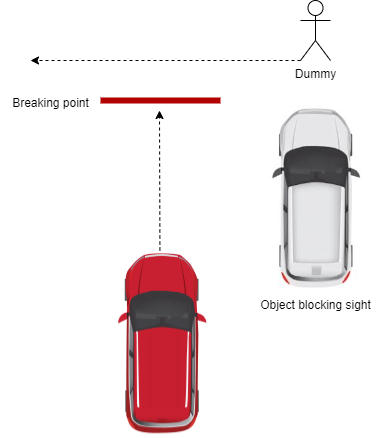
\includegraphics[scale=0.6,angle =0]{figure/test_illustration.png}
\caption{Illustration of the test, dummy walking in to the cars trajectory, red car is expected to emergency brake~\cite{EuroNCAP2021FILMPROTOCOL}. Source: Primary} 
\label{illustration_test}
\end{figure}

To guarantee proper execution of the test, it was crucial to adhere precisely to the established protocol~\cite{EuroNCAP2021FILMPROTOCOL}: \\

\begin{itemize}
    \item At the start of filming the car and the dummy representing a human should be in view with the dummy moving towards the camera. The camera should be positioned at an angle of approximately 45 degrees to the dummy motion. When the car is about to brake, the view should start to zoom in until the car has stopped.
    \item For at least half of the runs required under media films, a drone must be used in replacement of this view. Start filming following the car. When the car approaches the target, both the car and the target should be in view. The angle should be as perpendicular as possible to the car and target in order to show the action. \\
\end{itemize}
To achieve the goal of this project, several sub-tasks were identified: \\
\begin{itemize}
    \item Given the path of the object to be filmed, calculate a trajectory for the drone to document the test as outlined in~\cite{EuroNCAP2021FILMPROTOCOL}.
    \item Transfer the calculated trajectories using an existing protocol.
    \item Develop a mobile application capable of receiving the calculated trajectories.
    \item Parse the trajectories to formats accepted by the drone.
    \item Execute the test and fly with the given trajectories.
    \item Use the video stream from the drone to identify and track selected object, keeping it in the center of the frame at all times.
    \item Develop a graphical user interface (GUI) to display information about the drone, the video feed and its current status.
\end{itemize}
